\documentclass[aspectratio=169]{beamer}

% Shared Beamer settings for Applied Machine Learning lectures (UPES).
% Keep this file free of \documentclass to allow reuse via \input.

% Allow lecture sources to use shared theme/assets without copying them into each lecture folder.
% NOTE: These paths are relative to `Unit-xx/Lecture-yy/latex/` (and `Lab/Experiment-xx/latex/`).
\makeatletter
\def\input@path{{../../../_shared/}{../../../_shared/UPES-Beamer-Theme/}}
\makeatother

\usetheme{UPES}
\setbeamertemplate{navigation symbols}{}

\usepackage{amsmath}
\usepackage{amssymb}
\usepackage{booktabs}
\usepackage{graphicx}
\usepackage{hyperref}
\usepackage{xcolor}
\usepackage{listings}

% Code listings (Python-oriented for this subject).
\lstset{
  language=Python,
  basicstyle=\ttfamily\small,
  keywordstyle=\color{blue},
  commentstyle=\color{gray},
  stringstyle=\color{teal},
  showstringspaces=false,
  columns=fullflexible,
  breaklines=true
}

\usepackage{tikz}
\usetikzlibrary{arrows.meta,positioning,shapes.geometric,calc,fit,backgrounds}

% Per-slide source line (references shown on the slide itself).
\newcommand{\slidesources}[1]{%
  \vfill
  {\tiny\color{gray}\raggedright\sloppy\parbox{\linewidth}{Sources: #1}\par}%
}

% Unit-wise source strings for this subject (used by slides/notes).
% Path is relative to the lecture `latex/` folder (the compilation CWD).
% Source strings for Applied Machine Learning (CSAI2017P) — used by slides + notes.
% Prescribed texts and reference books are taken from the course syllabus.
% Support texts are the author-hosted open-access editions:
%   statlearning.com            (ISL with Python)
%   probml.github.io/pml-book   (Murphy, Probabilistic Machine Learning)
%   d2l.ai                      (Dive into Deep Learning)
%   mml-book.github.io          (Mathematics for Machine Learning)

\newcommand{\AMLRepoURL}{https://github.com/tali7c/Applied-Machine-Learning}

% --- prescribed -------------------------------------------------------------
\newcommand{\AMLPrescribed}{%
M\"uller and Guido, \textit{Introduction to Machine Learning with Python}, O'Reilly, 2016.;%
Bishop, \textit{Pattern Recognition and Machine Learning}, Springer, 2006.;%
Murphy, \textit{Machine Learning: A Probabilistic Perspective}, MIT Press, 2012.;%
Han, Kamber and Pei, \textit{Data Mining: Concepts and Techniques} (3e), Morgan Kaufmann, 2012.%
}

% --- unit-wise ---------------------------------------------------------------
\newcommand{\AMLUnitISources}{%
M\"uller and Guido, \textit{Introduction to Machine Learning with Python}, Ch. 1.;%
Bishop, \textit{Pattern Recognition and Machine Learning}, Ch. 1.;%
Murphy, \textit{Probabilistic Machine Learning: An Introduction}, MIT Press, 2022, Ch. 1.;%
Mitchell, \textit{Machine Learning}, McGraw Hill, 1997, Ch. 1.;%
Scikit-learn documentation, accessed 2026-08-04.%
}

\newcommand{\AMLUnitIISources}{%
Bishop, \textit{Pattern Recognition and Machine Learning}, \S1.5, \S4.3, \S7.1.;%
Zhang, Lipton, Li and Smola, \textit{Dive into Deep Learning}, \S3.4.;%
Shalev-Shwartz and Ben-David, \textit{Understanding Machine Learning}, Ch. 15.;%
Murphy, \textit{Probabilistic Machine Learning: An Introduction}, Ch. 5.%
}

\newcommand{\AMLUnitIIISources}{%
Zhang, Lipton, Li and Smola, \textit{Dive into Deep Learning}, Ch. 12 (Optimization Algorithms).;%
Deisenroth, Faisal and Ong, \textit{Mathematics for Machine Learning}, Ch. 7.;%
Kingma and Ba, ``Adam: A Method for Stochastic Optimization,'' ICLR 2015.;%
Ruder, ``An overview of gradient descent optimization algorithms,'' arXiv:1609.04747, 2016.%
}

\newcommand{\AMLUnitIVSources}{%
Han, Kamber and Pei, \textit{Data Mining: Concepts and Techniques} (3e), Ch. 3.;%
M\"uller and Guido, \textit{Introduction to Machine Learning with Python}, Ch. 3--4.;%
James, Witten, Hastie, Tibshirani and Taylor, \textit{An Introduction to Statistical Learning with Python}, Ch. 5--6, 12.;%
Scikit-learn documentation (preprocessing, model selection), accessed 2026-08-04.%
}

\newcommand{\AMLUnitVSources}{%
James et al., \textit{An Introduction to Statistical Learning with Python}, Ch. 3--6.;%
Bishop, \textit{Pattern Recognition and Machine Learning}, Ch. 3.;%
Deisenroth, Faisal and Ong, \textit{Mathematics for Machine Learning}, Ch. 9.;%
M\"uller and Guido, \textit{Introduction to Machine Learning with Python}, \S2.3.%
}

\newcommand{\AMLUnitVISources}{%
Han, Kamber and Pei, \textit{Data Mining: Concepts and Techniques} (3e), Ch. 8--9.;%
James et al., \textit{An Introduction to Statistical Learning with Python}, Ch. 8--9.;%
Bishop, \textit{Pattern Recognition and Machine Learning}, Ch. 4--5, 7, 14.;%
Zhang et al., \textit{Dive into Deep Learning}, Ch. 5.%
}

\newcommand{\AMLUnitVIISources}{%
Han, Kamber and Pei, \textit{Data Mining: Concepts and Techniques} (3e), Ch. 10.;%
James et al., \textit{An Introduction to Statistical Learning with Python}, Ch. 12.;%
M\"uller and Guido, \textit{Introduction to Machine Learning with Python}, \S3.5.;%
Ester, Kriegel, Sander and Xu, ``A density-based algorithm for discovering clusters (DBSCAN),'' KDD 1996.%
}

\newcommand{\AMLLabSources}{%
M\"uller and Guido, \textit{Introduction to Machine Learning with Python}, companion notebooks.;%
McKinney, \textit{Python for Data Analysis} (3e), O'Reilly, 2022.;%
Scikit-learn user guide, accessed 2026-08-04.;%
Matplotlib and Seaborn documentation, accessed 2026-08-04.%
}



\graphicspath{{../figures/}{../images/}{../../../_shared/}{../../../_shared/UPES-Beamer-Theme/}}

\title[Applied Machine Learning]{Applied Machine Learning}
\subtitle{Unit 03 -- Lecture 03: Gradient Descent}
\author{Tofik Ali}
\institute{School of Computer Science, UPES Dehradun}
\date{Autumn 2026}

% ---- a compact "output" block so code and its result sit together ----------
\lstdefinestyle{outblk}{
  basicstyle=\ttfamily\scriptsize\color{black!75},
  backgroundcolor=\color{black!5}, frame=leftline, framerule=2pt,
  rulecolor=\color{black!30}, breaklines=true, columns=fullflexible,
  xleftmargin=4pt, aboveskip=1pt, belowskip=1pt, literate={-}{{-}}1}
\lstnewenvironment{outblk}{\lstset{style=outblk}}{}

\begin{document}

\UPESCoverFrame
\setcounter{framenumber}{0}

\begin{frame}
  \titlepage
  \vspace{0.3em}
  \begin{center}
    \footnotesize Stochastic, mini-batch and momentum\\[0.25em]
    \footnotesize Topic focus: \textbf{how is the loss actually minimised?}\\[0.25em]
    \footnotesize Repository: \texttt{\AMLRepoURL}
  \end{center}
  \slidesources{\AMLUnitIIISources}
\end{frame}

\begin{frame}{Quick Links}
  \centering
  \hyperlink{sec:gd}{\beamerbutton{Gradient descent}}\hspace{0.5em}
  \hyperlink{sec:lr}{\beamerbutton{Learning rate}}\hspace{0.5em}
  \hyperlink{sec:sgd}{\beamerbutton{Stochastic}}\hspace{0.5em}
  \hyperlink{sec:mini}{\beamerbutton{Mini-batch}}\hspace{0.5em}
  \hyperlink{sec:mom}{\beamerbutton{Momentum}}\hspace{0.5em}
  \hyperlink{sec:summary}{\beamerbutton{Summary}}
\end{frame}

\begin{frame}{Agenda}
  \tableofcontents
\end{frame}

\begin{frame}{How this lecture works}
  \begin{columns}[T]
    \begin{column}{0.48\textwidth}
      \begin{block}{Every idea appears twice}
        \begin{enumerate}
          \item \textbf{By hand} --- small numbers, on paper, so you see the
            mechanism.
          \item \textbf{In code} --- the same thing, so you see the library does
            exactly that and nothing magic.
        \end{enumerate}
      \end{block}
    \end{column}
    \begin{column}{0.48\textwidth}
      \begin{alertblock}{Commit before you look}
        Four slides ask you to predict an answer before it is revealed. Write
        your guess down. Being wrong on paper is how the idea sticks.
      \end{alertblock}
    \end{column}
  \end{columns}
  \vspace{0.4em}
  \begin{center}
    \small Full derivations, more worked examples and 10 practice questions
    with solutions are in \texttt{notes.pdf}.
  \end{center}
\end{frame}

\begin{frame}[shrink=4]{Where we are}
  \begin{columns}[T]
    \begin{column}{0.46\textwidth}
      \begin{block}{Unit II gave us}
        \textbf{What} quantity do we minimise? MSE, MAE, Huber,
        cross-entropy, hinge.
      \end{block}
      \begin{exampleblock}{Unit III (today)}
        \textbf{How} do we minimise it?
      \end{exampleblock}
      \begin{block}{Next lecture}
        The adaptive optimisers: Adagrad, RMSprop, Adam.
      \end{block}
    \end{column}
    \begin{column}{0.5\textwidth}
      \begin{alertblock}{Why the separation matters}
        The algorithms in this lecture do not care which loss you chose. One
        optimiser, every model. That is why it was worth answering the two
        questions separately.
      \end{alertblock}
    \end{column}
  \end{columns}
\end{frame}

% =====================================================================
\section[GD]{Gradient descent}
\label{sec:gd}

\begin{frame}{Step 3, at last}
  \begin{enumerate}
    \item<1-> Propose a family of candidate models, controlled by parameters.
    \item<2-> Define \textbf{one number} saying how badly a candidate does.
      \hfill{\small\color{gray}(Unit II)}
    \item<3-> \textbf{Search the parameters to make that number small.}
      \hfill{\small\color{gray}(today)}
  \end{enumerate}
  \vspace{0.8em}
  \onslide<4->{
  \begin{exampleblock}{The whole of Unit III is one line}
    \centering \Large Step downhill. Repeat.
  \end{exampleblock}}
  \vspace{0.3em}
  \onslide<5->{
  \begin{center}\small
    Everything interesting is in three questions: \textbf{how big} a step,
    computed from \textbf{how much data}, and with \textbf{how much memory} of
    the last step.
  \end{center}}
\end{frame}

\begin{frame}[shrink=5]{Why not just solve it exactly?}
  For linear regression with squared error we can:
  $w^\star = (X^\top X)^{-1} X^\top y$.
  \vspace{0.5em}
  \begin{columns}[T]
    \begin{column}{0.32\textwidth}
      \begin{block}{Cost}
        $O(np^2 + p^3)$. At $p = 10^6$, $p^3 = 10^{18}$ operations.
      \end{block}
    \end{column}
    \begin{column}{0.32\textwidth}
      \begin{block}{Generality}
        Exists only because squared error is quadratic. Logistic loss: no
        closed form.
      \end{block}
    \end{column}
    \begin{column}{0.32\textwidth}
      \begin{block}{Memory}
        Needs all $n$ rows at once. Streams and big data do not oblige.
      \end{block}
    \end{column}
  \end{columns}
  \vspace{0.6em}
  \begin{alertblock}{The trade}
    Gradient descent swaps an exact answer computed \emph{once} for an
    approximate answer improved \emph{many times}. That is the only trade that
    scales.
  \end{alertblock}
\end{frame}

\begin{frame}{The derivative already tells you which way to go}
  \begin{columns}[T]
    \begin{column}{0.52\textwidth}
      \begin{itemize}
        \item $f'(w) > 0$: going right raises $f$ $\Rightarrow$ move
          \textbf{left}.
        \item $f'(w) < 0$: going right lowers $f$ $\Rightarrow$ move
          \textbf{right}.
      \end{itemize}
      \vspace{0.5em}
      Both say: move along $-f'(w)$.
    \end{column}
    \begin{column}{0.44\textwidth}
      \begin{exampleblock}{The algorithm}
        \centering\Large $w \leftarrow w - \eta\, f'(w)$
      \end{exampleblock}
    \end{column}
  \end{columns}
  \vspace{0.7em}
  \begin{center}
    $\eta$ is the \textbf{learning rate}. With $p$ parameters, replace $f'$ by
    the gradient: \quad $w \leftarrow w - \eta\,\nabla J(w)$.
  \end{center}
  \vspace{0.4em}
  \begin{center}\small
    Least squares: $\nabla J(w) = \frac{2}{n} X^\top (Xw - y)$. That is all the
    calculus this lecture needs.
  \end{center}
\end{frame}

\begin{frame}{By hand: five steps on $f(w)=(w-3)^2$}
  $f'(w) = 2(w-3)$, \quad $w_0 = 0$, \quad $\eta = 0.1$, \quad so
  $w \leftarrow 0.8\,w + 0.6$.
  \begin{center}\small
  \begin{tabular}{@{}rrrr@{}}
    \toprule
    $k$ & $w_k$ & $f(w_k)$ & $f'(w_k)$\\
    \midrule
    0 & 0.0000 & 9.0000 & $-6.0000$\\
    1 & 0.6000 & 5.7600 & $-4.8000$\\
    2 & 1.0800 & 3.6864 & $-3.8400$\\
    3 & 1.4640 & 2.3593 & $-3.0720$\\
    4 & 1.7712 & 1.5099 & $-2.4576$\\
    \bottomrule
  \end{tabular}
  \end{center}
  \vspace{0.2em}
  \begin{alertblock}{Look at the last column}
    \small $-6.0,\ -4.8,\ -3.84,\ -3.072$ --- every step is exactly $0.8$ times
    the one before. The algorithm brakes on its own as it approaches.
  \end{alertblock}
\end{frame}

\begin{frame}[fragile]{The same thing in code}
\begin{lstlisting}
def f(w):  return (w - 3.0)**2
def df(w): return 2.0*(w - 3.0)

eta, w = 0.1, 0.0
for k in range(5):
    print("k=%d  w=%.4f  f(w)=%.4f  f'(w)=%+.4f" % (k, w, f(w), df(w)))
    w = w - eta*df(w)
\end{lstlisting}
\begin{outblk}
k=0  w=0.0000  f(w)=9.0000  f'(w)=-6.0000
k=1  w=0.6000  f(w)=5.7600  f'(w)=-4.8000
k=2  w=1.0800  f(w)=3.6864  f'(w)=-3.8400
k=3  w=1.4640  f(w)=2.3593  f'(w)=-3.0720
k=4  w=1.7712  f(w)=1.5099  f'(w)=-2.4576
\end{outblk}
\end{frame}

\begin{frame}[shrink=6]{Where the $0.8$ comes from}
  \begin{columns}[T]
    \begin{column}{0.50\textwidth}
      Write $e_k = w_k - 3$ for the remaining error:
      \[
        e_{k+1} = (1-2\eta)\,e_k
        \;\Longrightarrow\;
        e_k = (1-2\eta)^k e_0 .
      \]
      With $\eta = 0.1$ the multiplier is $0.8$, so
      $w_k = 3 - 3(0.8)^k$ --- which prints exactly the table.
    \end{column}
    \begin{column}{0.48\textwidth}
      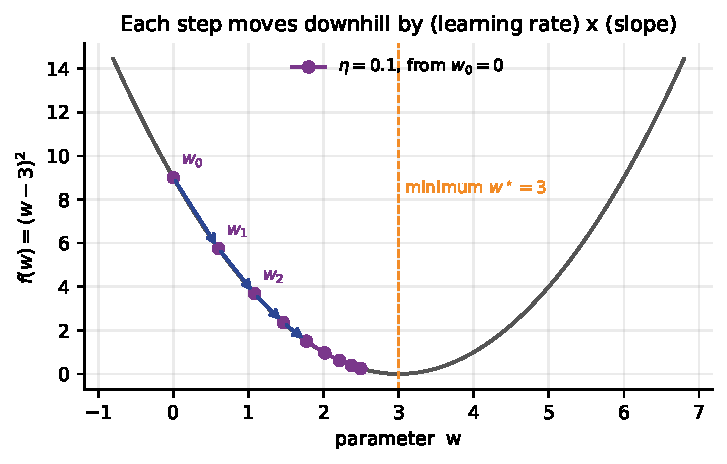
\includegraphics[width=\textwidth]{gdsteps.pdf}
    \end{column}
  \end{columns}
  \vspace{0.3em}
  \begin{alertblock}{Convergence is geometric, not linear}
    \small Each step buys the same \emph{percentage} of the remaining error,
    never the same amount. That is why every loss curve is a cliff followed by
    a long flat tail --- and why the last decimal place costs the most.
  \end{alertblock}
\end{frame}

% =====================================================================
\section[Step size]{The learning rate}
\label{sec:lr}

\begin{frame}[shrink=6]{Four regimes, from one formula}
  The error multiplier is $\lvert 1 - \eta f''\rvert$. Everything follows.
  \begin{center}\small
  \begin{tabular}{@{}llp{6.6cm}@{}}
    \toprule
    \textbf{Regime} & \textbf{Multiplier} & \textbf{Behaviour}\\
    \midrule
    $\eta$ too small      & just under $1$ & converges, but takes forever\\[2pt]
    $\eta$ well chosen    & near $0$       & converges fast, monotonically\\[2pt]
    $\eta$ too large      & in $(-1,0)$    & converges, overshooting and oscillating\\[2pt]
    $\eta$ past the limit & $>1$ in size   & \textbf{diverges}\\
    \bottomrule
  \end{tabular}
  \end{center}
  \vspace{0.3em}
  \begin{exampleblock}{The stability threshold}
    \centering
    $0 < \eta < \dfrac{2}{L}$, \quad $L$ = the largest curvature of $J$.
    \quad For $(w-3)^2$: $L = 2$, so $\eta < 1$.
  \end{exampleblock}
\end{frame}

\begin{frame}[fragile]{Predict first \#1}
Same problem, $w_0=0$, twenty iterations. $\eta < 1$ converges,
$\eta > 1$ diverges.

\begin{center}
  \textbf{What happens at $\eta$ exactly $1.00$?
  And at $\eta = 1.05$, five per cent past it?}
\end{center}
\vspace{0.3em}
\onslide<2->
\begin{outblk}
eta=0.10   |1-2*eta| = 0.80   w_20 =       2.9654
eta=0.50   |1-2*eta| = 0.00   w_20 =       3.0000
eta=0.90   |1-2*eta| = 0.80   w_20 =       2.9654
eta=1.00   |1-2*eta| = 1.00   w_20 =       0.0000
eta=1.05   |1-2*eta| = 1.10   w_20 =     -17.1825
\end{outblk}
\onslide<3->
\begin{alertblock}{At $\eta=1$ it bounces $0 \to 6 \to 0$ forever}
  \footnotesize Neutral: never converges, never diverges. Five per cent more
  and it is at $-17.18$ and accelerating. \textbf{There is no graceful
  degradation.}
\end{alertblock}
\end{frame}

\begin{frame}[shrink=10]{Two surprises, drawn}
  \begin{center}
    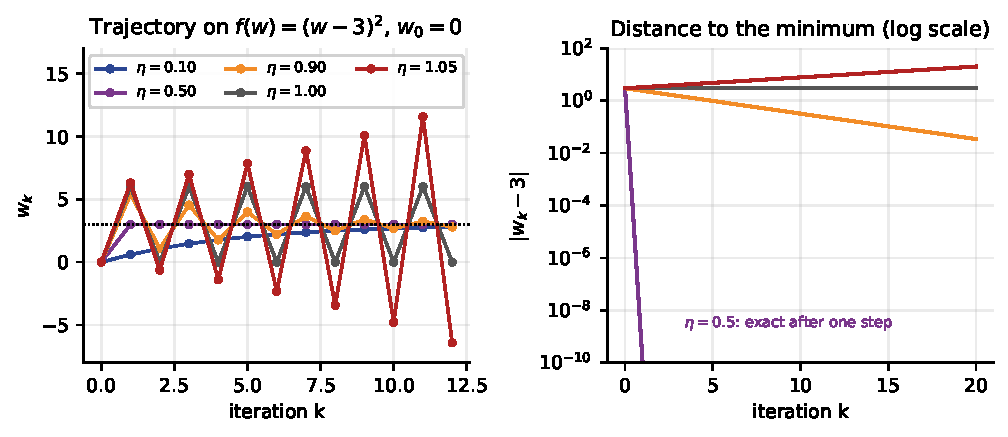
\includegraphics[width=0.80\textwidth]{lrgrid.pdf}
  \end{center}
  \begin{columns}[T]
    \begin{column}{0.47\textwidth}
      \begin{block}{$\eta = 0.50$ is exact in one step}
        \small The multiplier is \emph{zero}. For a quadratic, $\eta = 1/L$ is
        Newton's method.
      \end{block}
    \end{column}
    \begin{column}{0.47\textwidth}
      \begin{block}{$\eta = 0.10$ and $\eta = 0.90$ tie}
        \small Both give multiplier $0.8$ and reach $2.9654$. Nine times the
        learning rate bought nothing.
      \end{block}
    \end{column}
  \end{columns}
\end{frame}

\begin{frame}[shrink=4]{Diagnosing $\eta$ from a loss curve}
  \begin{center}\small
  \begin{tabular}{@{}p{6.2cm}p{6.4cm}@{}}
    \toprule
    \textbf{What you see} & \textbf{What to do}\\
    \midrule
    Still falling steeply when you stop & $\eta$ too small: multiply by 3, or train longer\\[3pt]
    Falls fast, then flattens & Healthy. Leave it alone\\[3pt]
    Falls, then bounces without settling & $\eta$ slightly too large --- or the SGD noise floor (later)\\[3pt]
    Rises, or becomes \texttt{nan} & Past the threshold. Divide $\eta$ by 10\\
    \bottomrule
  \end{tabular}
  \end{center}
  \vspace{0.4em}
  \begin{alertblock}{A good $\eta$ is a property of your data}
    $L$ depends on how your features are scaled. A learning rate that works on
    standardised data can be hopeless on raw data --- and we can measure
    exactly how hopeless.
  \end{alertblock}
\end{frame}

\begin{frame}[fragile]{Feature scaling is an optimisation decision}
One feature recorded in metres instead of kilometres --- multiply column 0 by
1000, change nothing else:
\begin{lstlisting}
Xbad = load_diabetes().data.copy()
Xbad[:, 0] *= 1000.0
evb = np.linalg.eigvalsh(2.0/n * (Xbad.T @ Xbad))
\end{lstlisting}
\begin{outblk}
condition number, standardised             470.1
condition number, one feature x1000   1.168e+08
stability limit 2/L, standardised         0.2485
stability limit 2/L, unscaled          4.420e-04
\end{outblk}
\onslide<2->
\begin{alertblock}{The usable learning rate fell by a factor of 562}
  \footnotesize And iterations scale with the condition number, so the run got
  about $250{,}000\times$ longer. \textbf{Standardise before you optimise.}
\end{alertblock}
\end{frame}

% =====================================================================
\section[SGD]{Stochastic gradient descent}
\label{sec:sgd}

\begin{frame}[fragile]{Batch gradient descent, on real data}
\texttt{load\_diabetes}: 442 patients, 10 features, both standardised.
\begin{lstlisting}
w = np.zeros(p)
for epoch in range(1, 6):
    w = w - 0.005*grad(X, y, w)         # grad = 2/n * X.T @ (X@w - y)
    print("epoch %2d   MSE %.4f" % (epoch, mse(X, y, w)))
\end{lstlisting}
\begin{outblk}
epoch  1   MSE 0.9713
epoch  2   MSE 0.9447
epoch  3   MSE 0.9199
epoch  4   MSE 0.8969
epoch  5   MSE 0.8754
least-squares optimum  MSE 0.4823
\end{outblk}
\begin{center}\small
  \textbf{Epoch} = one pass. \textbf{Update} = one application of the rule.
  Batch GD: \textbf{one update per epoch}, cost $O(np)$.
\end{center}
\end{frame}

\begin{frame}[shrink=9]{The structure we have been ignoring}
  \[
    J(w) = \frac{1}{n}\sum_{i=1}^{n} \ell_i(w)
    \qquad\Longrightarrow\qquad
    \nabla J(w) = \frac{1}{n}\sum_{i=1}^{n} \nabla \ell_i(w)
  \]
  \vspace{0.1em}
  \begin{center}
    The cost is an \textbf{average}. To estimate an average you do not need
    every term --- you need a \emph{sample}.
  \end{center}
  \vspace{0.5em}
  \begin{exampleblock}{Pick one example $i$ at random}
    \centering
    $\mathbb{E}_i\big[\nabla \ell_i(w)\big] = \nabla J(w)$ \quad --- an
    \textbf{unbiased} estimate, at $1/n$ the cost.
  \end{exampleblock}
  \vspace{0.4em}
  \begin{center}\Large
    $w \leftarrow w - \eta\,\nabla \ell_i(w)$
  \end{center}
  \begin{center}\small
    In one pass, SGD makes $n$ updates where batch GD makes one --- for the
    same total arithmetic.
  \end{center}
\end{frame}

\begin{frame}[shrink=10]{By hand: three points, one epoch}
  Predict $\hat y = wx$ with $x = (1,2,3)$, $y = (2,4,7)$, $w_0 = 0$,
  $\eta = 0.05$. Gradient of one example: $2x_i(wx_i - y_i)$.
  \begin{columns}[T]
    \begin{column}{0.42\textwidth}
      \begin{block}{One batch step}
        $\nabla J(0) = \frac{1}{3}(-4 -16 -42) = -20.67$\\[0.3em]
        $w \leftarrow 0 + 0.05(20.67) = \mathbf{1.0333}$
      \end{block}
    \end{column}
    \begin{column}{0.54\textwidth}
      \begin{block}{One epoch of SGD}
        \small
        \begin{tabular}{@{}llr@{}}
          $x=1$: & $2(1)(0-2) = -4.00$      & $w = 0.2000$\\
          $x=2$: & $2(2)(0.4-4) = -14.40$   & $w = 0.9200$\\
          $x=3$: & $2(3)(2.76-7) = -25.44$  & $w = \mathbf{2.1920}$\\
        \end{tabular}
      \end{block}
    \end{column}
  \end{columns}
  \vspace{0.3em}
  \begin{alertblock}{Exact optimum: $w^\star = 31/14 = 2.2143$}
    \small Identical arithmetic --- three per-example gradients either way.
    Batch reached $1.03$; SGD reached $2.19$, within one per cent. SGD's second
    gradient was evaluated at $w=0.2$, not at $w=0$.
  \end{alertblock}
\end{frame}

\begin{frame}[fragile]{The same thing in code}
\begin{lstlisting}
w = 0.0
g = np.mean(2*xs*(w*xs - ys))
print("one full-batch step:  gradient %+.4f  ->  w = %.4f" % (g, w - eta*g))
w = 0.0                                       # now one epoch of SGD
for xi, yi in zip(xs, ys):
    gi = 2*xi*(w*xi - yi); w = w - eta*gi
    print("  SGD on x=%.0f:      gradient %+.4f  ->  w = %.4f" % (xi, gi, w))
\end{lstlisting}
\begin{outblk}
one full-batch step:  gradient -20.6667  ->  w = 1.0333
  SGD on x=1:      gradient -4.0000  ->  w = 0.2000
  SGD on x=2:      gradient -14.4000  ->  w = 0.9200
  SGD on x=3:      gradient -25.4400  ->  w = 2.1920
\end{outblk}
\begin{center}\small
  Optimum $2.2143$. In practice \textbf{shuffle every epoch}.
\end{center}
\end{frame}

\begin{frame}[fragile]{The price: SGD never quite arrives}
Unbiased is not noiseless. Near the optimum the full gradient vanishes but the
per-example ones do not, so SGD orbits in a cloud whose size grows with $\eta$.
\begin{lstlisting}
eta = eta0/(1 + 0.002*t) if decay else eta0    # Robbins-Monro schedule
\end{lstlisting}
\begin{outblk}
SGD (B=1, 30 epochs), constant step 0.02   MSE 0.5395
SGD (B=1, 30 epochs), decayed step         MSE 0.4834
least-squares optimum                      MSE 0.4823
\end{outblk}
\onslide<2->
\begin{alertblock}{$\sum \eta_t = \infty$ and $\sum \eta_t^2 < \infty$}
  \footnotesize The first says do not stop before arriving; the second says
  damp the noise. $\eta_t = \eta_0/(1+ct)$ does both --- and closed almost the
  whole remaining gap here.
\end{alertblock}
\end{frame}

% =====================================================================
\section[Mini-batch]{Mini-batch gradient descent}
\label{sec:mini}

\begin{frame}{Nothing forces $B$ to be $1$ or $n$}
  \[
    w \;\leftarrow\; w \;-\; \eta \,\frac{1}{B}\sum_{i \in \mathcal{B}}
      \nabla \ell_i(w),
    \qquad \mathcal{B} \text{ random, } \lvert \mathcal{B}\rvert = B
  \]
  \vspace{0.3em}
  \begin{center}
  \begin{tabular}{@{}lcccc@{}}
    \toprule
    & $B$ & updates/epoch & noise & cost/update\\
    \midrule
    Batch      & $n$          & $1$   & none     & $O(np)$\\
    Mini-batch & $32$--$512$  & $n/B$ & moderate & $O(Bp)$\\
    Stochastic & $1$          & $n$   & large    & $O(p)$\\
    \bottomrule
  \end{tabular}
  \end{center}
  \vspace{0.6em}
  \begin{center}\small
    Batch and SGD are the two endpoints. The answer is always in between ---
    and this section is why.
  \end{center}
\end{frame}

\begin{frame}[fragile]{Predict first \#2}
Thirty epochs, same $\eta$, same total arithmetic per epoch. SGD reaches
MSE \textbf{0.5268} after \emph{one} epoch.

\begin{center}
  \textbf{How many epochs does full-batch gradient descent need to reach the
  same MSE?}
\end{center}
\vspace{0.4em}
\onslide<2->
\begin{outblk}
                updates/epoch   after 1 epoch   after 30 epochs
batch  B=442              1          0.9713            0.6219
mini   B= 32             14          0.7393            0.4860
SGD    B=  1            442          0.5268            0.4859
Full-batch GD needs 80 epochs to reach the same MSE.
\end{outblk}
\onslide<3->
\begin{center}\small
  \textbf{Eighty passes against one} (optimum $0.4823$). All of it comes from
  updating 442 times per pass instead of once.
\end{center}
\end{frame}

\begin{frame}[shrink=8]{Two panels that contradict each other --- both true}
  \begin{center}
    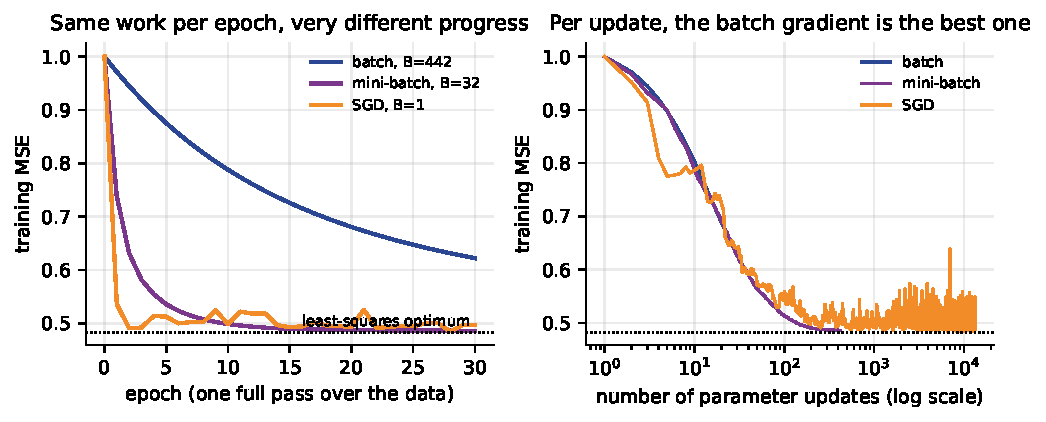
\includegraphics[width=0.84\textwidth]{epochs.pdf}
  \end{center}
  \begin{center}\small
    Per \textbf{update}, the batch gradient is the best one (right). Per unit
    of \textbf{work}, it is by far the worst (left). We are judged on the
    second, because work is what you pay for.
  \end{center}
\end{frame}

\begin{frame}[fragile]{How noisy is one example, really?}
\begin{lstlisting}
g_full = grad(X, y, w0)
for B in [1, 2, 4, 8, 16, 32, 64, 128, 256]:
    ...  # RMS of ||grad on a random batch of B  -  g_full||, 3000 draws
\end{lstlisting}
\begin{outblk}
|| full gradient ||  2.4157
B=   1   RMS ||g_B - g|| = 6.3234
B=   2   RMS ||g_B - g|| = 4.4099
B=   4   RMS ||g_B - g|| = 3.1309
B=   8   RMS ||g_B - g|| = 2.1805
B=  16   RMS ||g_B - g|| = 1.5199
B=  32   RMS ||g_B - g|| = 1.0641
\end{outblk}
\onslide<2->
\begin{alertblock}{Read the first two lines together}
  \footnotesize The true gradient has length $2.42$; a single-example gradient
  is typically wrong by $6.32$. \textbf{A single SGD step often points uphill.}
  It works only because the errors cancel.
\end{alertblock}
\end{frame}

\begin{frame}[shrink=6]{The $1/\sqrt{B}$ law}
  \begin{columns}[T]
    \begin{column}{0.52\textwidth}
      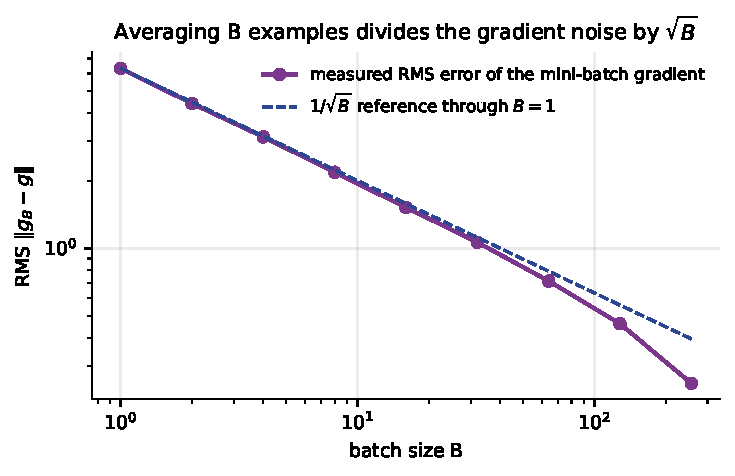
\includegraphics[width=\textwidth]{gradnoise.pdf}
    \end{column}
    \begin{column}{0.44\textwidth}
      \begin{block}{Each doubling of $B$}
        multiplies the error by $1/\sqrt{2} = 0.707$:\\
        $6.32 \to 4.41 \to 3.13 \to 2.18$
      \end{block}
      \begin{alertblock}{The decisive trade}
        Noise falls as $\sqrt{B}$; cost grows as $B$. Doubling $B$ buys
        $41\%$ less noise for $100\%$ more work.
      \end{alertblock}
      \small $B{=}1 \to B{=}32$: $32\times$ the work, $5.9\times$ less noise
      ($\sqrt{32} = 5.66$).
    \end{column}
  \end{columns}
\end{frame}

\begin{frame}[fragile]{Predict first \#3}
$B=32$ does $32\times$ the arithmetic per update that $B=1$ does. Both reach
essentially the same MSE (0.4860 against 0.4859 after 30 epochs).

\begin{center}
  \textbf{Per epoch --- identical total arithmetic --- which is faster in
  wall-clock time, and by how much?}
\end{center}
\vspace{0.4em}
\onslide<2->
\begin{outblk}
B=   1   442 updates/epoch     1.224 ms per epoch
B=  32    14 updates/epoch     0.040 ms per epoch
B= 442     1 updates/epoch     0.005 ms per epoch
\end{outblk}
\onslide<3->
\begin{alertblock}{$B=32$ is 31 times faster than $B=1$}
  \footnotesize Same arithmetic, one vectorised matrix operation instead of 32
  tiny ones. On a GPU the effect is far larger --- thousands of cores sit idle
  processing one example at a time.
\end{alertblock}
\end{frame}

\begin{frame}[shrink=10]{Why mini-batch wins}
  \begin{columns}[T]
    \begin{column}{0.47\textwidth}
      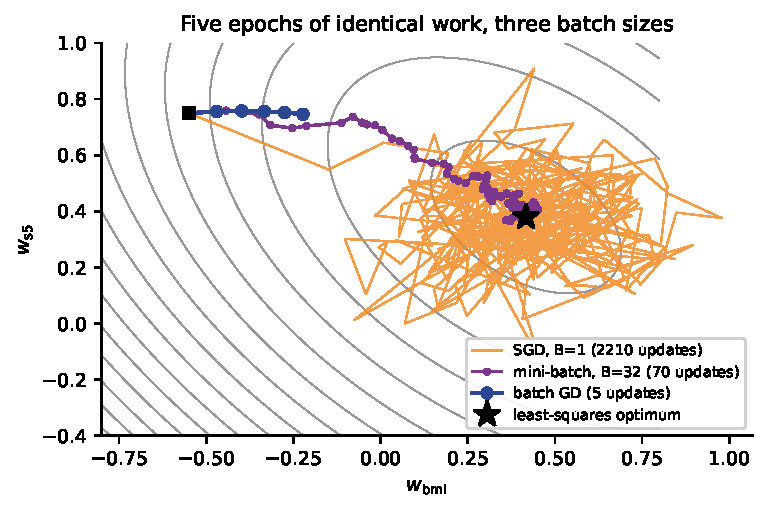
\includegraphics[width=\textwidth]{sgdpath.pdf}\\[0.2em]
      {\scriptsize Five epochs of identical work. Batch GD barely leaves the
      start; SGD arrives fast, then rattles around the optimum.}
    \end{column}
    \begin{column}{0.49\textwidth}
      \begin{exampleblock}{Better than both ends, not a compromise}
        \small
        \begin{itemize}
          \item Keeps almost all of SGD's update frequency --- 14 per epoch was
            enough here.
          \item Recovers vectorised arithmetic: $31\times$ on this laptop, far
            more on a GPU.
          \item Cuts gradient noise by $\sqrt{B}$ into the bargain.
        \end{itemize}
      \end{exampleblock}
      \begin{alertblock}{Terminology in the wild}
        \small Almost everything called ``SGD'' is mini-batch GD.
        \textbf{Start at $B=32$, powers of two, tune $\eta$ first.}
      \end{alertblock}
    \end{column}
  \end{columns}
\end{frame}

% =====================================================================
\section{Momentum}
\label{sec:mom}

\begin{frame}{The ravine}
  \begin{columns}[T]
    \begin{column}{0.5\textwidth}
      \begin{block}{Measured on our data}
        Largest curvature $8.05$, smallest $0.017$.\\[0.3em]
        \textbf{Condition number $\kappa = 470$.}
      \end{block}
      \vspace{0.2em}
      A long, narrow valley: steep walls, gently sloping floor.
    \end{column}
    \begin{column}{0.46\textwidth}
      \begin{alertblock}{The bind}
        $\eta < 2/L$ is set by the \textbf{steep walls}.\\[0.3em]
        The progress you want is along the \textbf{floor}, where the curvature
        is $470$ times smaller.
      \end{alertblock}
    \end{column}
  \end{columns}
  \vspace{0.6em}
  \begin{center}
    So the iterates bounce from wall to wall and creep along the valley.
  \end{center}
  \vspace{0.2em}
  \begin{center}\small
    \textbf{Gradient descent is limited by the direction you do not want to
    travel in.}
  \end{center}
\end{frame}

\begin{frame}{The heavy ball}
  Stop thinking of a hiker taking independent steps. Think of a ball rolling.
  \vspace{0.4em}
  \begin{center}
  \begin{tabular}{@{}ll@{}}
    \toprule
    \textbf{Along the floor} & slope points the same way $\Rightarrow$ velocity
      \emph{builds}\\
    \textbf{Across the valley} & slope reverses each step $\Rightarrow$
      contributions \emph{cancel}\\
    \bottomrule
  \end{tabular}
  \end{center}
  \vspace{0.6em}
  \begin{exampleblock}{Polyak's heavy ball --- the form PyTorch and D2L use}
    \centering\Large
    $v \leftarrow \beta v + \nabla J(w)$ \qquad
    $w \leftarrow w - \eta\, v$
  \end{exampleblock}
  \vspace{0.3em}
  \begin{center}\small
    $\beta = 0$ recovers plain gradient descent exactly.
  \end{center}
\end{frame}

\begin{frame}{Momentum is an exponentially weighted average}
  Unroll it from $v_0 = 0$:
  \[
    v_t = \beta v_{t-1} + g_t
        = g_t + \beta g_{t-1} + \beta^2 g_{t-2} + \cdots
        = \sum_{j\ge 0} \beta^{\,j} g_{t-j}
  \]
  \vspace{0.1em}
  \begin{center}
    Total weight $= \displaystyle\sum_{j \ge 0}\beta^{\,j} = \frac{1}{1-\beta}$
  \end{center}
  \vspace{0.5em}
  \begin{exampleblock}{The number to memorise}
    \centering\Large
    $\eta_{\text{eff}} \approx \dfrac{\eta}{1-\beta}$
    \qquad
    {\normalsize $\beta = 0.9 \Rightarrow 10\eta$; \quad
                 $\beta = 0.99 \Rightarrow 100\eta$}
  \end{exampleblock}
  \vspace{0.3em}
  \begin{center}\small
    A $10\times$ speed-up in consistent directions, without raising $\eta$ in
    the inconsistent ones.
  \end{center}
\end{frame}

\begin{frame}[shrink=8]{By hand: four steps of momentum}
  $f(w) = (w-3)^2$, \; $\eta = 0.1$, \; $\beta = 0.9$, \; $w_0 = 0$, $v_0 = 0$.
  \begin{center}\small
  \begin{tabular}{@{}rrll@{}}
    \toprule
    $k$ & $g_k$ & $v_k = 0.9\,v_{k-1} + g_k$ & $w_k = w_{k-1} - 0.1\,v_k$\\
    \midrule
    1 & $-6.0000$ & $-6.0000$   & $0 + 0.6000 = 0.6000$\\
    2 & $-4.8000$ & $-10.2000$  & $0.6 + 1.0200 = 1.6200$\\
    3 & $-2.7600$ & $-11.9400$  & $1.62 + 1.1940 = 2.8140$\\
    4 & $-0.3720$ & $-11.1180$  & $2.814 + 1.1118 = \mathbf{3.9258}$\\
    \bottomrule
  \end{tabular}
  \end{center}
  \vspace{0.2em}
  \begin{alertblock}{Plain GD was at $1.7712$ after four steps}
    \small Momentum is at $3.9258$ --- already \textbf{past} the minimum at
    $3$. Row 4 shows how: the gradient is nearly zero ($-0.372$) but the
    velocity is still $-11.12$. The ball arrives travelling fast.
  \end{alertblock}
\end{frame}

\begin{frame}[fragile]{Predict first \#4}
Same one-dimensional bowl, $\eta = 0.1$, starting at $w_0 = 0$ with the minimum
at $w = 3$. Plain GD reaches $\lvert w-3\rvert < 10^{-3}$ in 36 steps.

\begin{center}
  \textbf{With $\beta = 0.9$: faster or slower?
  And how far past $3$ does it go?}
\end{center}
\vspace{0.4em}
\onslide<2->
\begin{outblk}
beta=0.0   first k with |w-3|<1e-3:  36   highest w reached: 3.0000
beta=0.5   first k with |w-3|<1e-3:  20   highest w reached: 3.2092
beta=0.9   first k with |w-3|<1e-3:  92   highest w reached: 5.1269
\end{outblk}
\onslide<3->
\begin{alertblock}{$\beta = 0.9$ is two and a half times \emph{slower}}
  \footnotesize And it sails out to $5.13$ --- almost as far past the minimum
  as it started short of it. A 1-D quadratic has $\kappa = 1$: no ravine, so
  nothing for momentum to fix, and only the overshoot to pay for.
\end{alertblock}
\end{frame}

\begin{frame}[shrink=8]{Overshoot, drawn}
  \begin{center}
    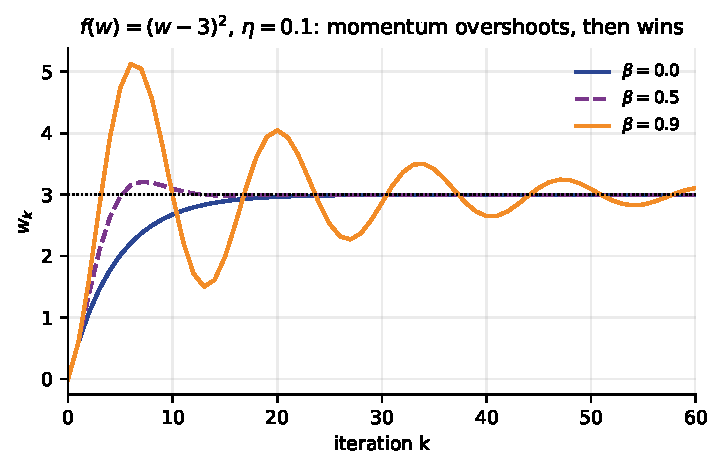
\includegraphics[width=0.62\textwidth]{momentum1d.pdf}
  \end{center}
  \begin{alertblock}{Momentum is not a free improvement}
    \small It is a targeted remedy for \textbf{ill-conditioned} problems ---
    which describes almost every real model, but not this one.
  \end{alertblock}
\end{frame}

\begin{frame}[fragile]{Now put it in a ravine}
$f(w) = 0.01 w_1^2 + 2 w_2^2$, so $\kappa = 4/0.02 = 200$. Plain GD's ceiling is
$2/L = 0.5$; we use $\eta = 0.475$ throughout.
\begin{outblk}
plain-GD ceiling      2/L          = 0.500
momentum ceiling  2(1+beta)/L      = 0.950   (beta=0.9)
eta=0.475  beta=0.0   iterations to ||w||<1e-3:  954
eta=0.475  beta=0.5   iterations to ||w||<1e-3:  467
eta=0.475  beta=0.9   iterations to ||w||<1e-3:  135
eta=0.900  beta=0.0   iterations to ||w||<1e-3:  diverged at k=20
eta=0.900  beta=0.9   iterations to ||w||<1e-3:  161
\end{outblk}
\onslide<2->
\begin{alertblock}{$954 \to 135$: a $7.1\times$ speed-up from one extra line}
  \footnotesize And the last two rows: at $\eta = 0.9$ plain GD explodes, while
  momentum converges --- because momentum's ceiling is
  $2(1+\beta)/L$, not $2/L$.
\end{alertblock}
\end{frame}

\begin{frame}[shrink=8]{The ravine, drawn --- and it is not what you expect}
  \begin{center}
    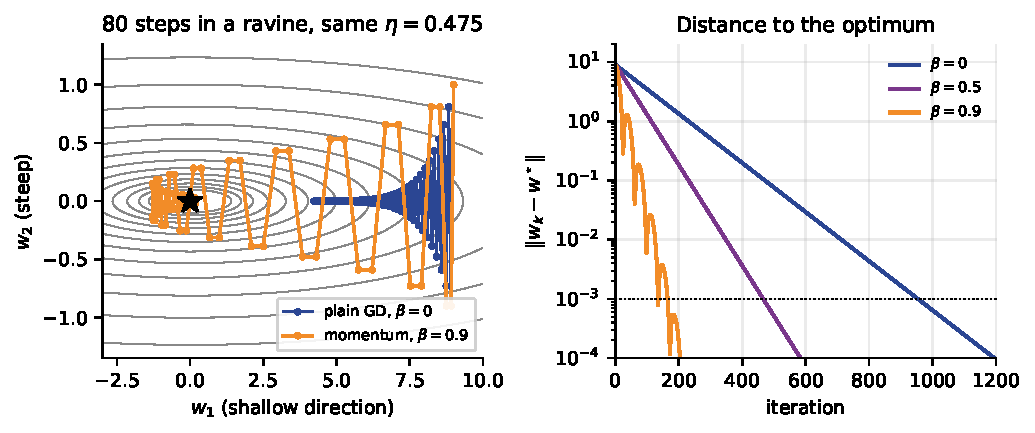
\includegraphics[width=0.86\textwidth]{ravine.pdf}
  \end{center}
  \begin{center}\small
    Momentum's path is \textbf{messier}, not smoother. What it is not, is
    stuck. It trades cross-valley tidiness for along-valley speed --- in a
    ravine, always a trade you want.
  \end{center}
\end{frame}

\begin{frame}[fragile]{On the real dataset, and with mini-batches}
\begin{outblk}
beta=0.0   eta=0.2361   full-batch iterations to the optimum:  1605
beta=0.9   eta=0.2361   full-batch iterations to the optimum:   128
\end{outblk}
\begin{center}\small
  $\kappa = 470$ on the diabetes problem, so $12.5\times$ --- more than the
  $7.1\times$ at $\kappa = 200$. \textbf{Worse conditioning, more benefit.}
\end{center}
\begin{outblk}
mini-batch B=32, eta=0.005, 5 epochs
   beta=0.00   MSE 0.5358
   beta=0.90   MSE 0.4870
   beta=0.99   MSE 0.5674
least-squares optimum   MSE 0.4823
\end{outblk}
\onslide<2->
\begin{center}\small
  $\beta = 0.99$ is \emph{worse than no momentum}: the effective step is
  $100\eta$ and the run overshoots.
\end{center}
\end{frame}

\begin{frame}[shrink=6]{Two things that will cost you an afternoon}
  \begin{alertblock}{When you raise $\beta$, lower $\eta$}
    Effective step is $\eta/(1-\beta)$. Moving $\beta$ from $0.9$ to $0.99$
    multiplies your learning rate by \textbf{ten} without you touching it.
    Rescale by $(1-\beta_{\text{new}})/(1-\beta_{\text{old}})$.
  \end{alertblock}
  \vspace{0.3em}
  \begin{alertblock}{Two conventions, differing by a factor of $1-\beta$}
    \begin{center}\small
    \begin{tabular}{@{}ll@{}}
      \toprule
      PyTorch, D2L, these slides & $v \leftarrow \beta v + g$\\
      Andrew Ng, the Adam paper  & $v \leftarrow \beta v + (1-\beta) g$\\
      \bottomrule
    \end{tabular}
    \end{center}
    \vspace{0.2em}
    Both correct; identical if $\eta$ is scaled by $1/(1-\beta)$. Copy $\eta$
    across without rescaling and your learning rate silently changes tenfold.
  \end{alertblock}
\end{frame}

% =====================================================================
\section{Summary}
\label{sec:summary}

\begin{frame}[shrink=12]{Summary}
  \begin{enumerate}\small
    \item $w \leftarrow w - \eta \nabla J(w)$. On a quadratic the error is
      multiplied by a fixed factor each step: convergence is \textbf{geometric}.
    \item Hard ceiling $\eta < 2/L$. At $\eta=1.00$ our run bounced forever; at
      $1.05$ it hit $-17.18$ in twenty steps. No graceful degradation.
    \item $\eta = 0.1$ and $\eta = 0.9$ converged at \emph{identical} rates.
      Bigger is not faster.
    \item The cost is an average, so one random example gives an
      \textbf{unbiased} gradient at $1/n$ the price. That is SGD.
    \item It is very noisy: true gradient length $2.42$, single-example error
      $6.32$. Steps often point uphill; the errors cancel.
    \item Per epoch, small batches win: SGD reached $0.5268$ in one epoch;
      batch GD needed \textbf{80}.
    \item Noise falls as $1/\sqrt{B}$, cost grows as $B$. $B{=}32$ measured
      $5.9\times$ less noise than $B{=}1$ for $32\times$ the arithmetic.
    \item \textbf{Mini-batch wins because it vectorises}: same MSE as $B{=}1$,
      $31\times$ faster per epoch.
    \item $v \leftarrow \beta v + \nabla J$: an exponentially weighted average,
      effective step $\eta/(1-\beta)$.
    \item Momentum \textbf{overshoots} --- to $5.13$ past a minimum at $3$ ---
      and on a well-conditioned problem it is slower.
    \item In a ravine it is transformative: $954 \to 135$ at $\kappa=200$,
      $1605 \to 128$ at $\kappa=470$. It also raises the ceiling to
      $2(1+\beta)/L$.
    \item Standardising cut $\kappa$ from $1.2\times10^8$ to $470$.
      Conditioning is something you control.
  \end{enumerate}
\end{frame}

\begin{frame}[shrink=3]{Before the next lecture}
  \begin{columns}[T]
    \begin{column}{0.48\textwidth}
      \begin{block}{Read}
        \texttt{notes.pdf} --- the full derivations, the Robbins--Monro
        conditions, and \textbf{10 practice questions with worked solutions}.
      \end{block}
      \begin{block}{Do}
        Questions 1, 6 and 10. Question 6 is momentum by hand; question 10 ties
        scaling, conditioning and the learning rate together.
      \end{block}
    \end{column}
    \begin{column}{0.48\textwidth}
      \begin{exampleblock}{Next: adaptive optimisers}
        Momentum gives every coordinate the same $\eta$ and the same
        $\beta$.\\[0.3em]
        L4 asks what happens when each coordinate gets its own step size:
        Adagrad, RMSprop, Adadelta, Adam.
      \end{exampleblock}
      \begin{alertblock}{T1 follows this lecture}
        Units I--II, 40 minutes.
      \end{alertblock}
    \end{column}
  \end{columns}
  \begin{center}
    \small Materials: \texttt{\AMLRepoURL}
  \end{center}
  \slidesources{\AMLUnitIIISources}
\end{frame}

\end{document}
